\chapter{Eletromiografia de Superfície}
\label{ch:sEMG}
\section{Definição}
A sEMG é o estudo relacionado às transformações elétricas das contrações musculares. É um exame indolor e não invasivo, por permitir a execução com mobilidade, dos movimentos musculares solicitados. A sEMG pode ser executada repetidas vezes sem causar um grande desconforto ao paciente, sendo rápida, livre de radiação e de fácil compreensão. Serve para analisar um grupo ou um feixe muscular específico \cite{de2010eletromiografia}, onde gera-se um sinal sEMG sobre a atividade muscular analisada.

Um sinal sEMG é obtido na medição das tensões relacionados as correntes elétricas, durante a contração muscular. Fornecendo assim em um intervalo de tempo, a média desta atividade neuromuscular \cite{reaz2006techniques}.

A sEMG caracteriza-se pela utilização de um dispositivo sobre a pele do paciente, o qual implica a detecção dos potenciais elétricos relativos às fibras musculares, ou seja, é possível detectar quando um músculo é ativado e qual o movimento foi executado, além de, relacionar a associação dos diferentes músculos envolvidos \cite{botelho2010avaliaccao}.

\section{Características do sinal}
Para melhor entender as características do sinal gerado pela sEMG, nesta seção é introduzido um breve resumo sobre os elementos que compõe a musculatura humana.

\subsection{Contração muscular}
O processo de ativação muscular começa com a liberação Acetilcolina (ACo - neurotransmissor que opera na comunicação de impulso nervoso do neurônio para as celulares musculares \cite{flores2005estructura} pelo axônio do neurônio motor até a ligação muscular. Esse neurotransmissor é liberado como consequência do potencial de ação pré-sináptico e resulta na excitação das fibras musculares no PEPS (Processo Pós-Sináptico) devido a abertura dos canais iónicos na membrana plasmática, no caso os receptores nicotínicos, através dos PEPS abertos canais de cálcio necessitantes de tensão elétrica se abrem provocando o potencial de ação pós-sináptico, que se propaga ao longo da fibra muscular \cite{da2005detecccao}.

A contração muscular ocorre com ligações químicas envolvendo cálcio (Ca2+) e as enzimas troponina, actina e miosina, com a liberação cálcio devido a despolarização nesse processo de propagação. Isto ocorre devido a ligação de cálcio a enzima troponina, que libera os sítios de ligação na actina para a miosina, provocando o encurtamento das fibras e logo a contração do músculo. A desconexão da miosina com a actina consume ATP (Adenosina Trifosfato), um nucleotídeo encarregado do armazenamento de energia nas ligações químicas \cite{da2005detecccao}.

O relaxamento muscular ocorre quando o cálcio é recapturado pelo retículo sarcoplasmático (retículo endoplasmático especializado no armazenamento de íons de cálcio), por uma bomba de ATP \cite{da2005detecccao}. 

\subsection{Unidade Motora}
Primeiramente temos a UM (Unidade Motora), uma coleção de fibras musculares inervadas por um único neurônio motor alfa, sendo a menor unidade operacional de um músculo, podendo ser ativada pelo controle neural. Na atividade muscular, ocorre a ativação do neurônio alfa dentro da UM, produzindo tensão nas fibras musculares ao passo que ocorre a propagação do sinal ao longo das fibras, o músculo é relaxado quando o neurônio alfa para a atividade \cite{yousefi2014characterizing}.

O PAUM (Potencial de Ação da Unidade Motora) é a soma dos potenciais de ação das contrações musculares em uma unidade motora relacionadas as tensões detectadas pelos eletrodos da sEMG e descrevem a soma de todas as UM ativas, ou seja, a soma de todos os PAUMs detectadas. Um conjunto de PAUMs que compõem a ação de um músculo é denominado de Trem de PAUM \cite{yousefi2014characterizing}. Um diagrama sobre o PAUM pode ser visto na Figura ~\ref{PAUM}.

A Figura ~\ref{UnidadeMotora}, representa um esquema simplificado da comunicação do neurônio com a UM do músculo.

\begin{figure}[!htb]
   \centering
    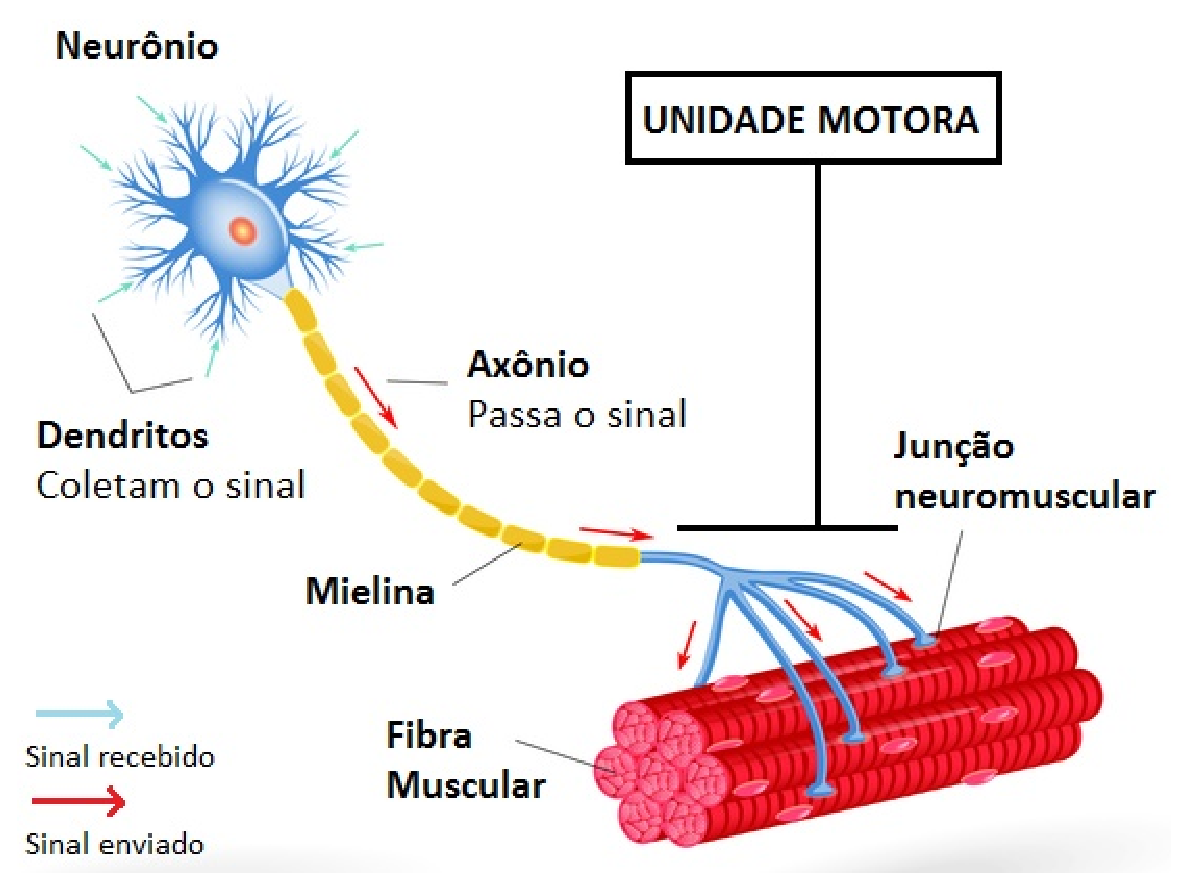
\includegraphics[width=0.8\textwidth]{figuras/motor-neuron.eps}
    \caption{Modelo de uma unidade motora, adaptado de \citeonline{Sabino}.}
    \label{UnidadeMotora}
\end{figure}

A equação ~\ref{eq:EMGT} descreve um sEMG. Um sEMG é a medida ao longo do tempo da contração de um MUP \textit{\textbf{m}}, de um total de \textit{\textbf{N, MUPs}}, a função \textit{\textbf{n(t)}} representa possíveis ruídos encontrados na coleta, ambas as funções são parametrizadas pelo tempo \cite{yousefi2014characterizing}.

\begin{equation} \label{eq:EMGT}
    EMG_{t} =\sum_{m=1}^{N} MUPs_{m}(t)+n(t)
\end{equation}

\begin{figure}[!htb]
    \centering
     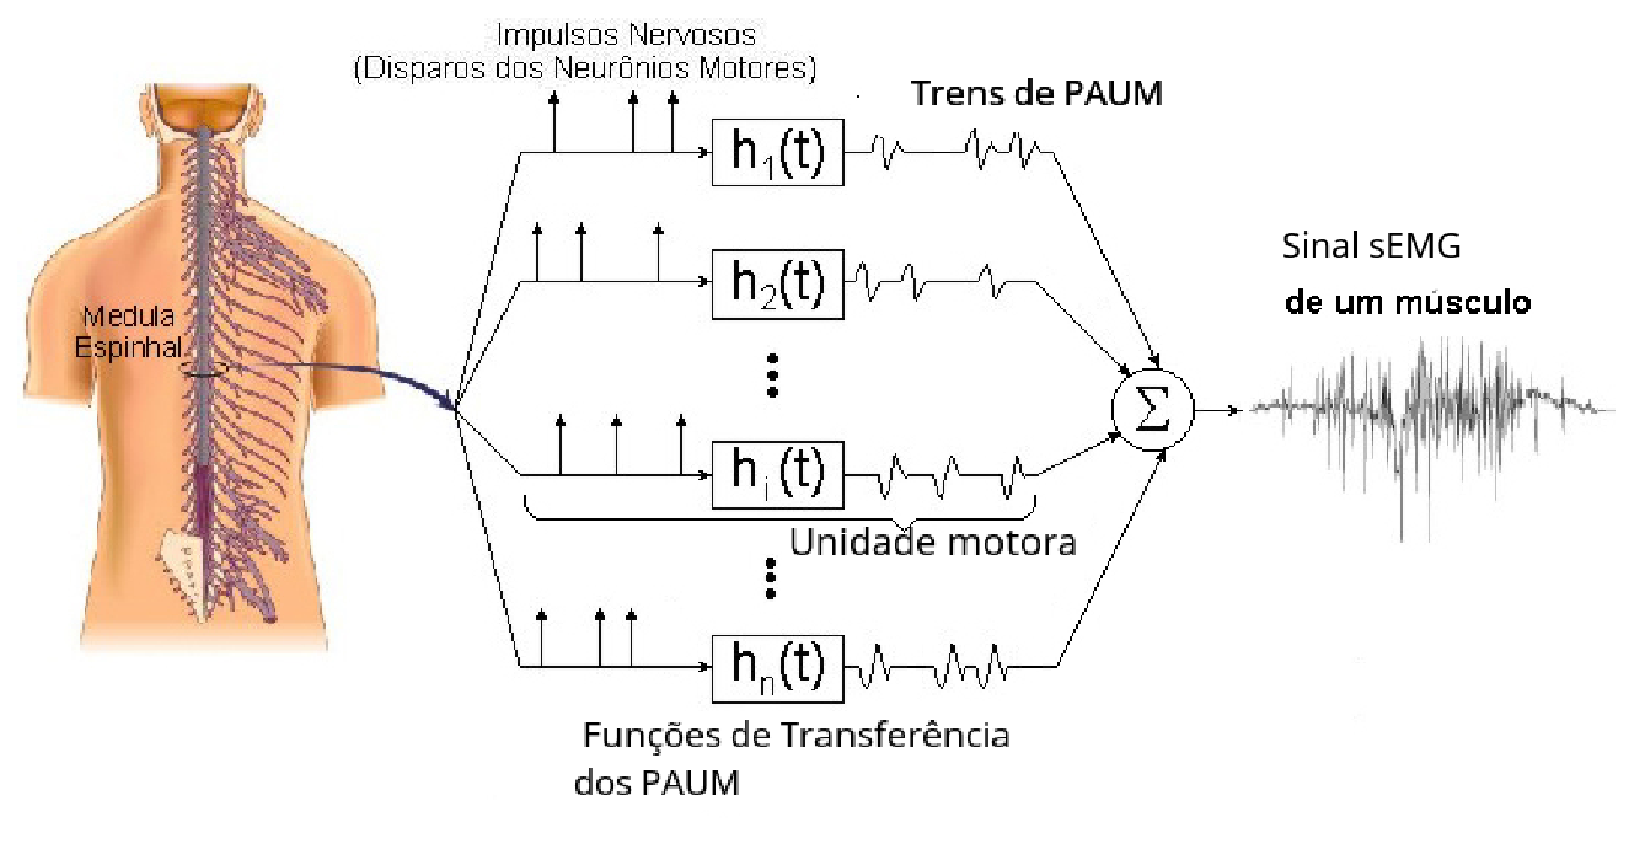
\includegraphics[width=0.9\textwidth]{figuras/Representacao-esquematica-da-geracao-do-Sinal-Mioeletrico-de-um-musculo-a-partir-da.eps}
     \caption{Sinal sEMG muscular, adaptado de \citeonline{Ortolan}.}
     \label{PAUM}
 \end{figure}

Este tipo de sinal inevitavelmente encontra ruído do equipamento e de outras fontes biológicas presentes no corpo do indivíduo, os quais interferem na coleta \cite{yousefi2014characterizing}.

Com relação a DP, o tremor de repouso é o sintoma mais comum, possuindo uma frequência entre 4 e 6 Hz.
\cite{jankovic2008parkinson}.

\section{Aplicações da sEMG}
A sEMG é largamente utilizada por profissionais de diversas áreas científicas que estudam o movimento humano, como médicos, fisioterapeutas, fonoaudiólogos e profissionais em educação física, sendo utilizada na análise clínica relacionada a ativação muscular, intensidade e duração durante a contração \cite{nascimento2012surface}. Tais informações podem ser utilizadas, por exemplo, no estudo da fadiga muscular em atletas \cite{schmitz2012unchanged} ou na detecção de doenças degenerativas como DP \cite{eftaxias2015detection}.